\chapter{Systemdesign og arkitektur}
\label{chap:architecture}

Dette kapitel beskriver systemets overordnede arkitektur og de centrale designbeslutninger, der ligger til grund for implementeringen. Kapitlet gennemgår systemets komponenter, deres indbyrdes relationer og de dataflows der forbinder dem.

\section{Overordnet systemarkitektur}
\label{sec:systemarkitektur}

Systemet er opbygget som en tre-lags klient-server-arkitektur bestående af en iOS-mobilapplikation, en Go-baseret middleware-server og to eksterne cloud-services. Figur~\ref{fig:system-overview} illustrerer de overordnede komponenter og deres kommunikation.

\begin{figure}[H]
  \centering
  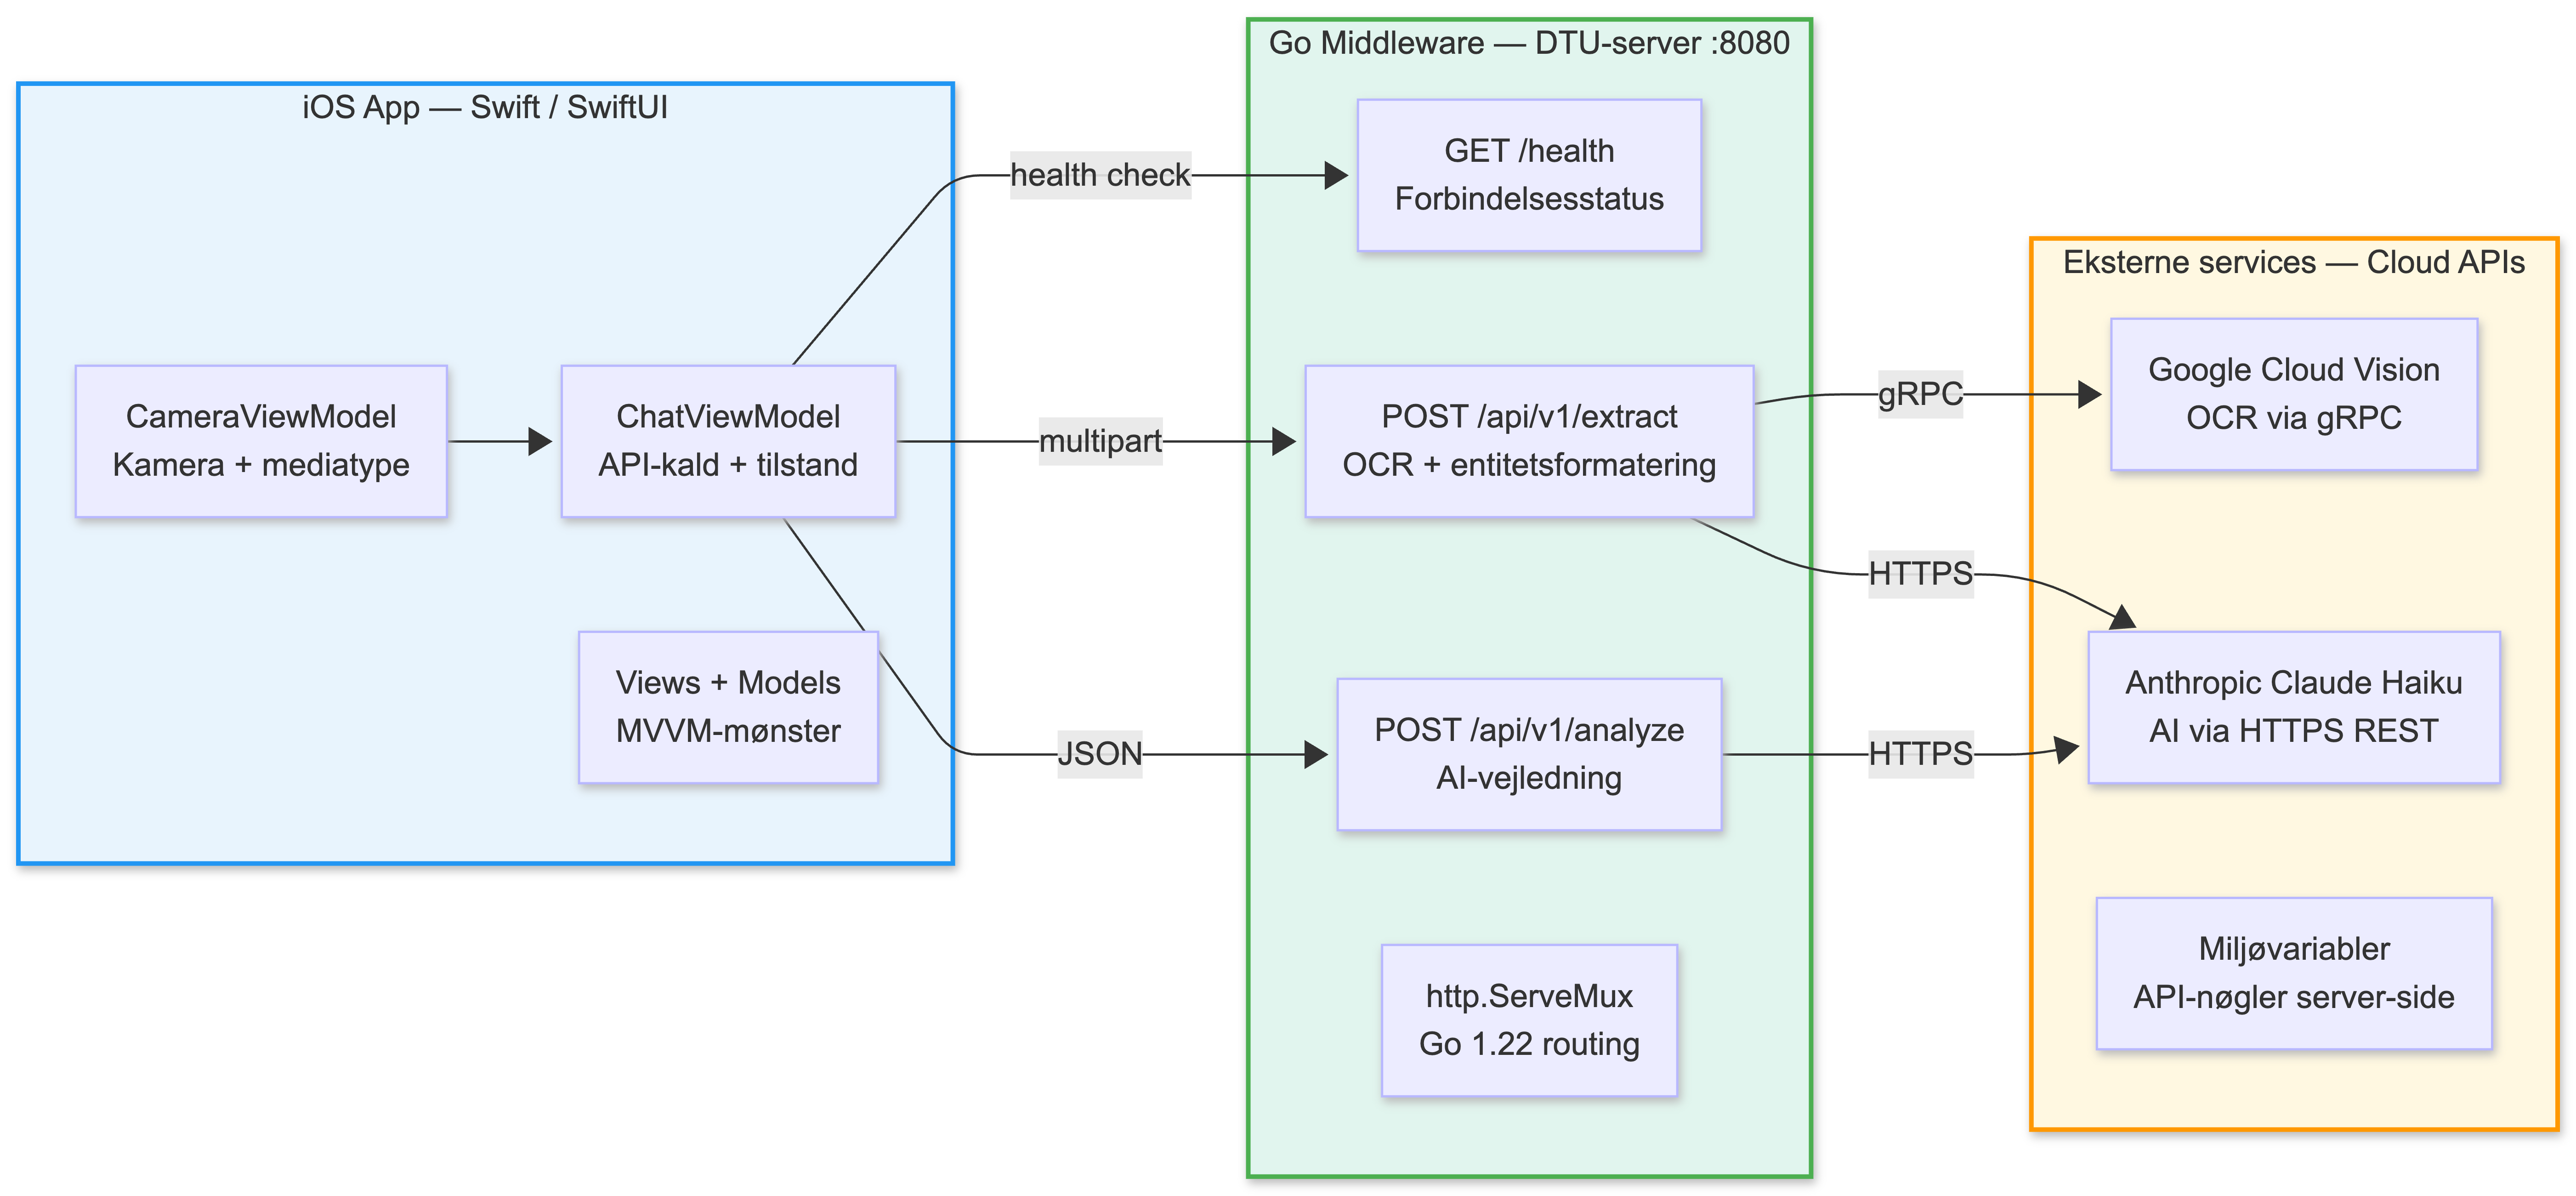
\includegraphics[width=\textwidth]{figures/Systemarkitektur.png}
  \caption{Overordnet systemarkitektur}
  \label{fig:system-overview}
\end{figure}


\textbf{iOS-applikationen} kører på teknikerens iPhone eller iPad og udgør brugergrænsefladen. Al logik i klientlaget er organiseret efter MVVM-mønstret (beskrevet i afsnit~\ref{sec:mvvm}). Kommunikation med serveren sker udelukkende via HTTP over det lokale netværk eller internet.

\textbf{Go middleware-serveren} er deployeret på en DTU-server (\texttt{130.225.170.229:8080}) og fungerer som det centrale orkestreringslag. Serveren modtager mediefiler fra klienten, koordinerer kald til eksterne AI-services og returnerer strukturerede svar til klienten. Ved at placere al AI-logik i middleware-laget undgås eksponering af API-nøgler i klientkoden, og det bliver muligt at udskifte individuelle services uden ændringer i iOS-applikationen.

\textbf{Google Cloud Vision} anvendes udelukkende til OCR-behandling af billeder og video-frames via gRPC-protokollen.

\textbf{Anthropic Claude Haiku} anvendes til to opgaver: strukturering af OCR-råtekst til typede entiteter og generering af vedligeholdelsesvejledning. Kommunikation sker via Anthropic's REST API over HTTPS.

\section{MVVM-arkitekturmønstret}
\label{sec:mvvm}

iOS-applikationen er struktureret efter MVVM-mønstret (Model-View-ViewModel), som adskiller brugergrænsefladen fra applikationens forretningslogik og datahåndtering~\cite{mvvm}. Figur~\ref{fig:mvvm} viser den konkrete mapping fra mønstret til applikationens komponenter.

\begin{figure}[H]
  \centering
  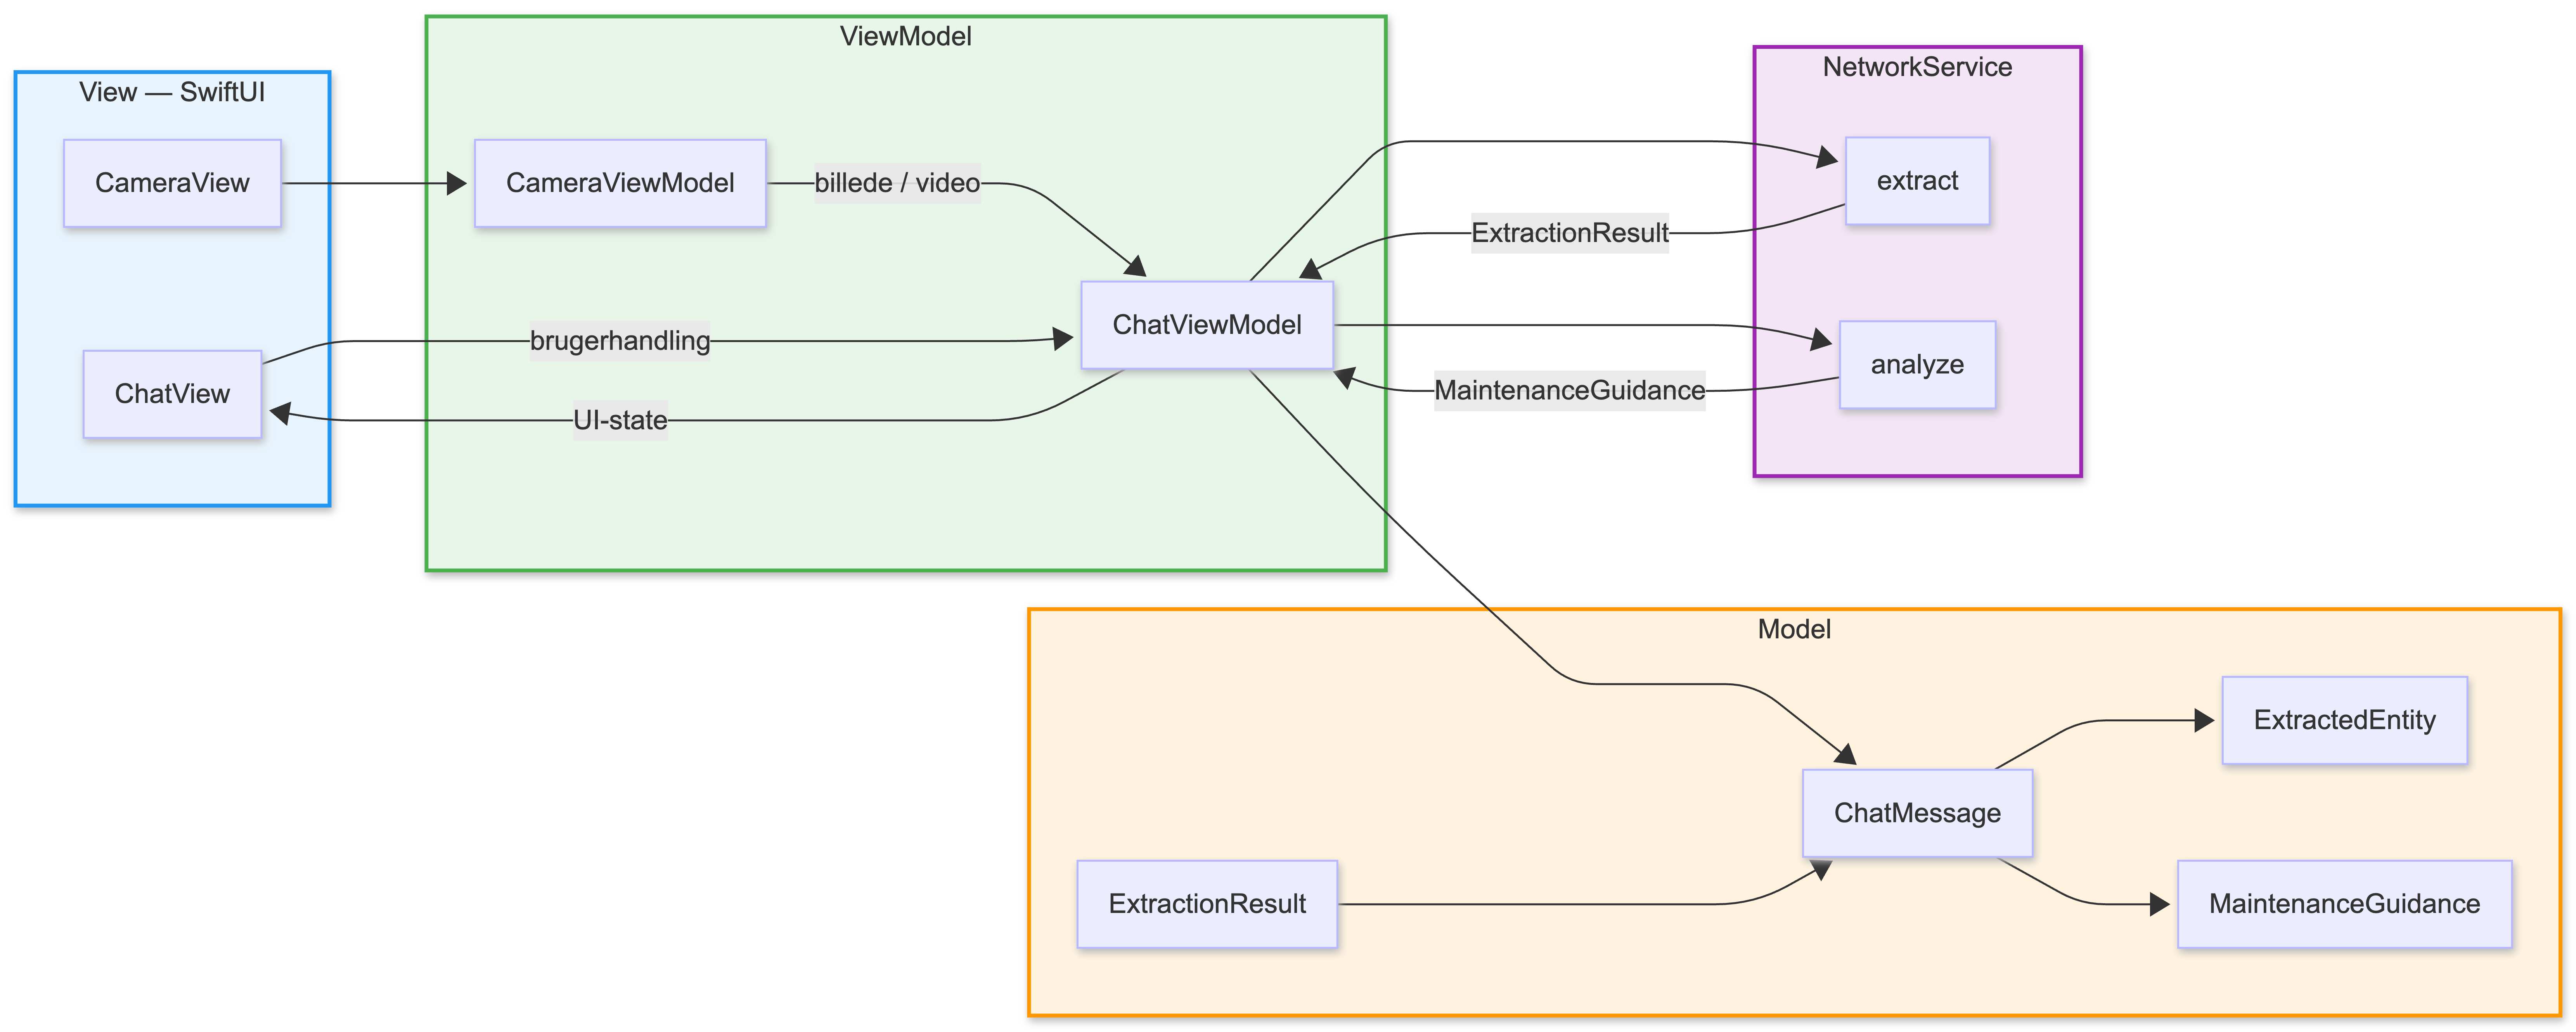
\includegraphics[width=0.85\textwidth]{figures/MVVM_final.png}
  \caption{MVVM-arkitektur i iOS-applikationen}
  \label{fig:mvvm}
\end{figure}

\textbf{Model-laget} repræsenterer applikationens datastrukturer. De centrale modeller er:

\begin{itemize}
  \item \texttt{ChatMessage} — en besked i chatten med en tilhørende \texttt{MessageKind}-enum der dækker seks tilstande: \texttt{text}, \texttt{extractedEntities}, \texttt{guidance}, \texttt{flagged}, \texttt{loading} og \texttt{error}
  \item \texttt{ExtractedEntity} — én identificeret entitet fra OCR-resultatet med label, værdi og tilladte handlinger
  \item \texttt{MaintenanceGuidance} — den strukturerede vedligeholdelsesvejledning returneret af Claude
  \item \texttt{ExtractionResult} — det samlede resultat af et extract-kald med entiteter, råtekst, confidence og review-flag
\end{itemize}

\textbf{ViewModel-laget} indeholder applikationens logik og fungerer som bindeled mellem View-laget og \texttt{NetworkService}:

\begin{itemize}
  \item \texttt{ChatViewModel} er annoteret med \texttt{@MainActor} og eksponerer \texttt{@Published}-properties til View-laget. ViewModellen implementerer et \textit{placeholder-replace-pattern}: når en netværksoperation startes, indsættes en loading-besked med et foruddefineret ID, som efterfølgende erstattes in-place af det endelige svar. Dette eliminerer flimmer i UI'et og bevarer beskedhistorikken intakt.
  \item \texttt{CameraViewModel} håndterer tilstanden for kamera-flowet, herunder valg af medie (billede eller video) og navigation til chat-visningen.
\end{itemize}

\textbf{NetworkService} fungerer som applikationens netværkslag og er det 
eneste sted der kommunikerer direkte med Go-middlewaren. \texttt{ChatViewModel} 
kalder \texttt{NetworkService.shared.extract()} og 
\texttt{NetworkService.shared.analyze()} via Swift's \texttt{async/await}, 
og \texttt{NetworkService} returnerer henholdsvis \texttt{ExtractionResult} 
og \texttt{MaintenanceGuidance} til \texttt{ChatViewModel}.


\textbf{View-laget} er implementeret i SwiftUI og består primært af \texttt{ChatView}, \texttt{CameraView} og et system af seks beskedbubble-typer, der renderer de forskellige \texttt{MessageKind}-tilstande.

\section{API-design}
\label{sec:api-design}

Middleware-serverens REST API eksponerer fire endpoints, som er opsummeret i tabel~\ref{tab:api-endpoints}.

\begin{table}[H]
  \centering
  \caption{API-endpoints på Go middleware-serveren}
  \label{tab:api-endpoints}
  \begin{tabularx}{\textwidth}{@{}llX@{}}
    \toprule
    \textbf{Metode} & \textbf{Endpoint} & \textbf{Beskrivelse} \\
    \midrule
    \texttt{GET}  & \texttt{/health}          & Returnerer serverens status og tidsstempel. Anvendes af iOS-klienten til at vise forbindelsesstatus i realtid \\
    \addlinespace
    \texttt{GET}  & \texttt{/version}         & Returnerer API-versionsnummer \\
    \addlinespace
    \texttt{POST} & \texttt{/api/v1/extract}  & Modtager et billede eller en video som \texttt{multipart/form-data}, kører OCR og returnerer strukturerede entiteter som JSON \\
    \addlinespace
    \texttt{POST} & \texttt{/api/v1/analyze}  & Modtager en valgt entitet med kontekst som JSON og returnerer struktureret vedligeholdelsesvejledning \\
    \bottomrule
  \end{tabularx}
\end{table}

Routingen implementeres via Go 1.22's indbyggede \texttt{http.ServeMux} med method-prefixed patterns, eksempelvis \texttt{"POST /api/v1/extract"}, hvilket eliminerer behovet for tredjeparts routing-biblioteker og giver klar adskillelse af HTTP-metoder på compilerniveau.

\section{Dataflow: Billedbaseret udtræk}
\label{sec:dataflow-billede}

Figur~\ref{fig:flow-image} viser det komplette dataflow for det primære use case: upload af et billede og udtræk af maskinentiteter.

\begin{figure}[H]
  \centering
  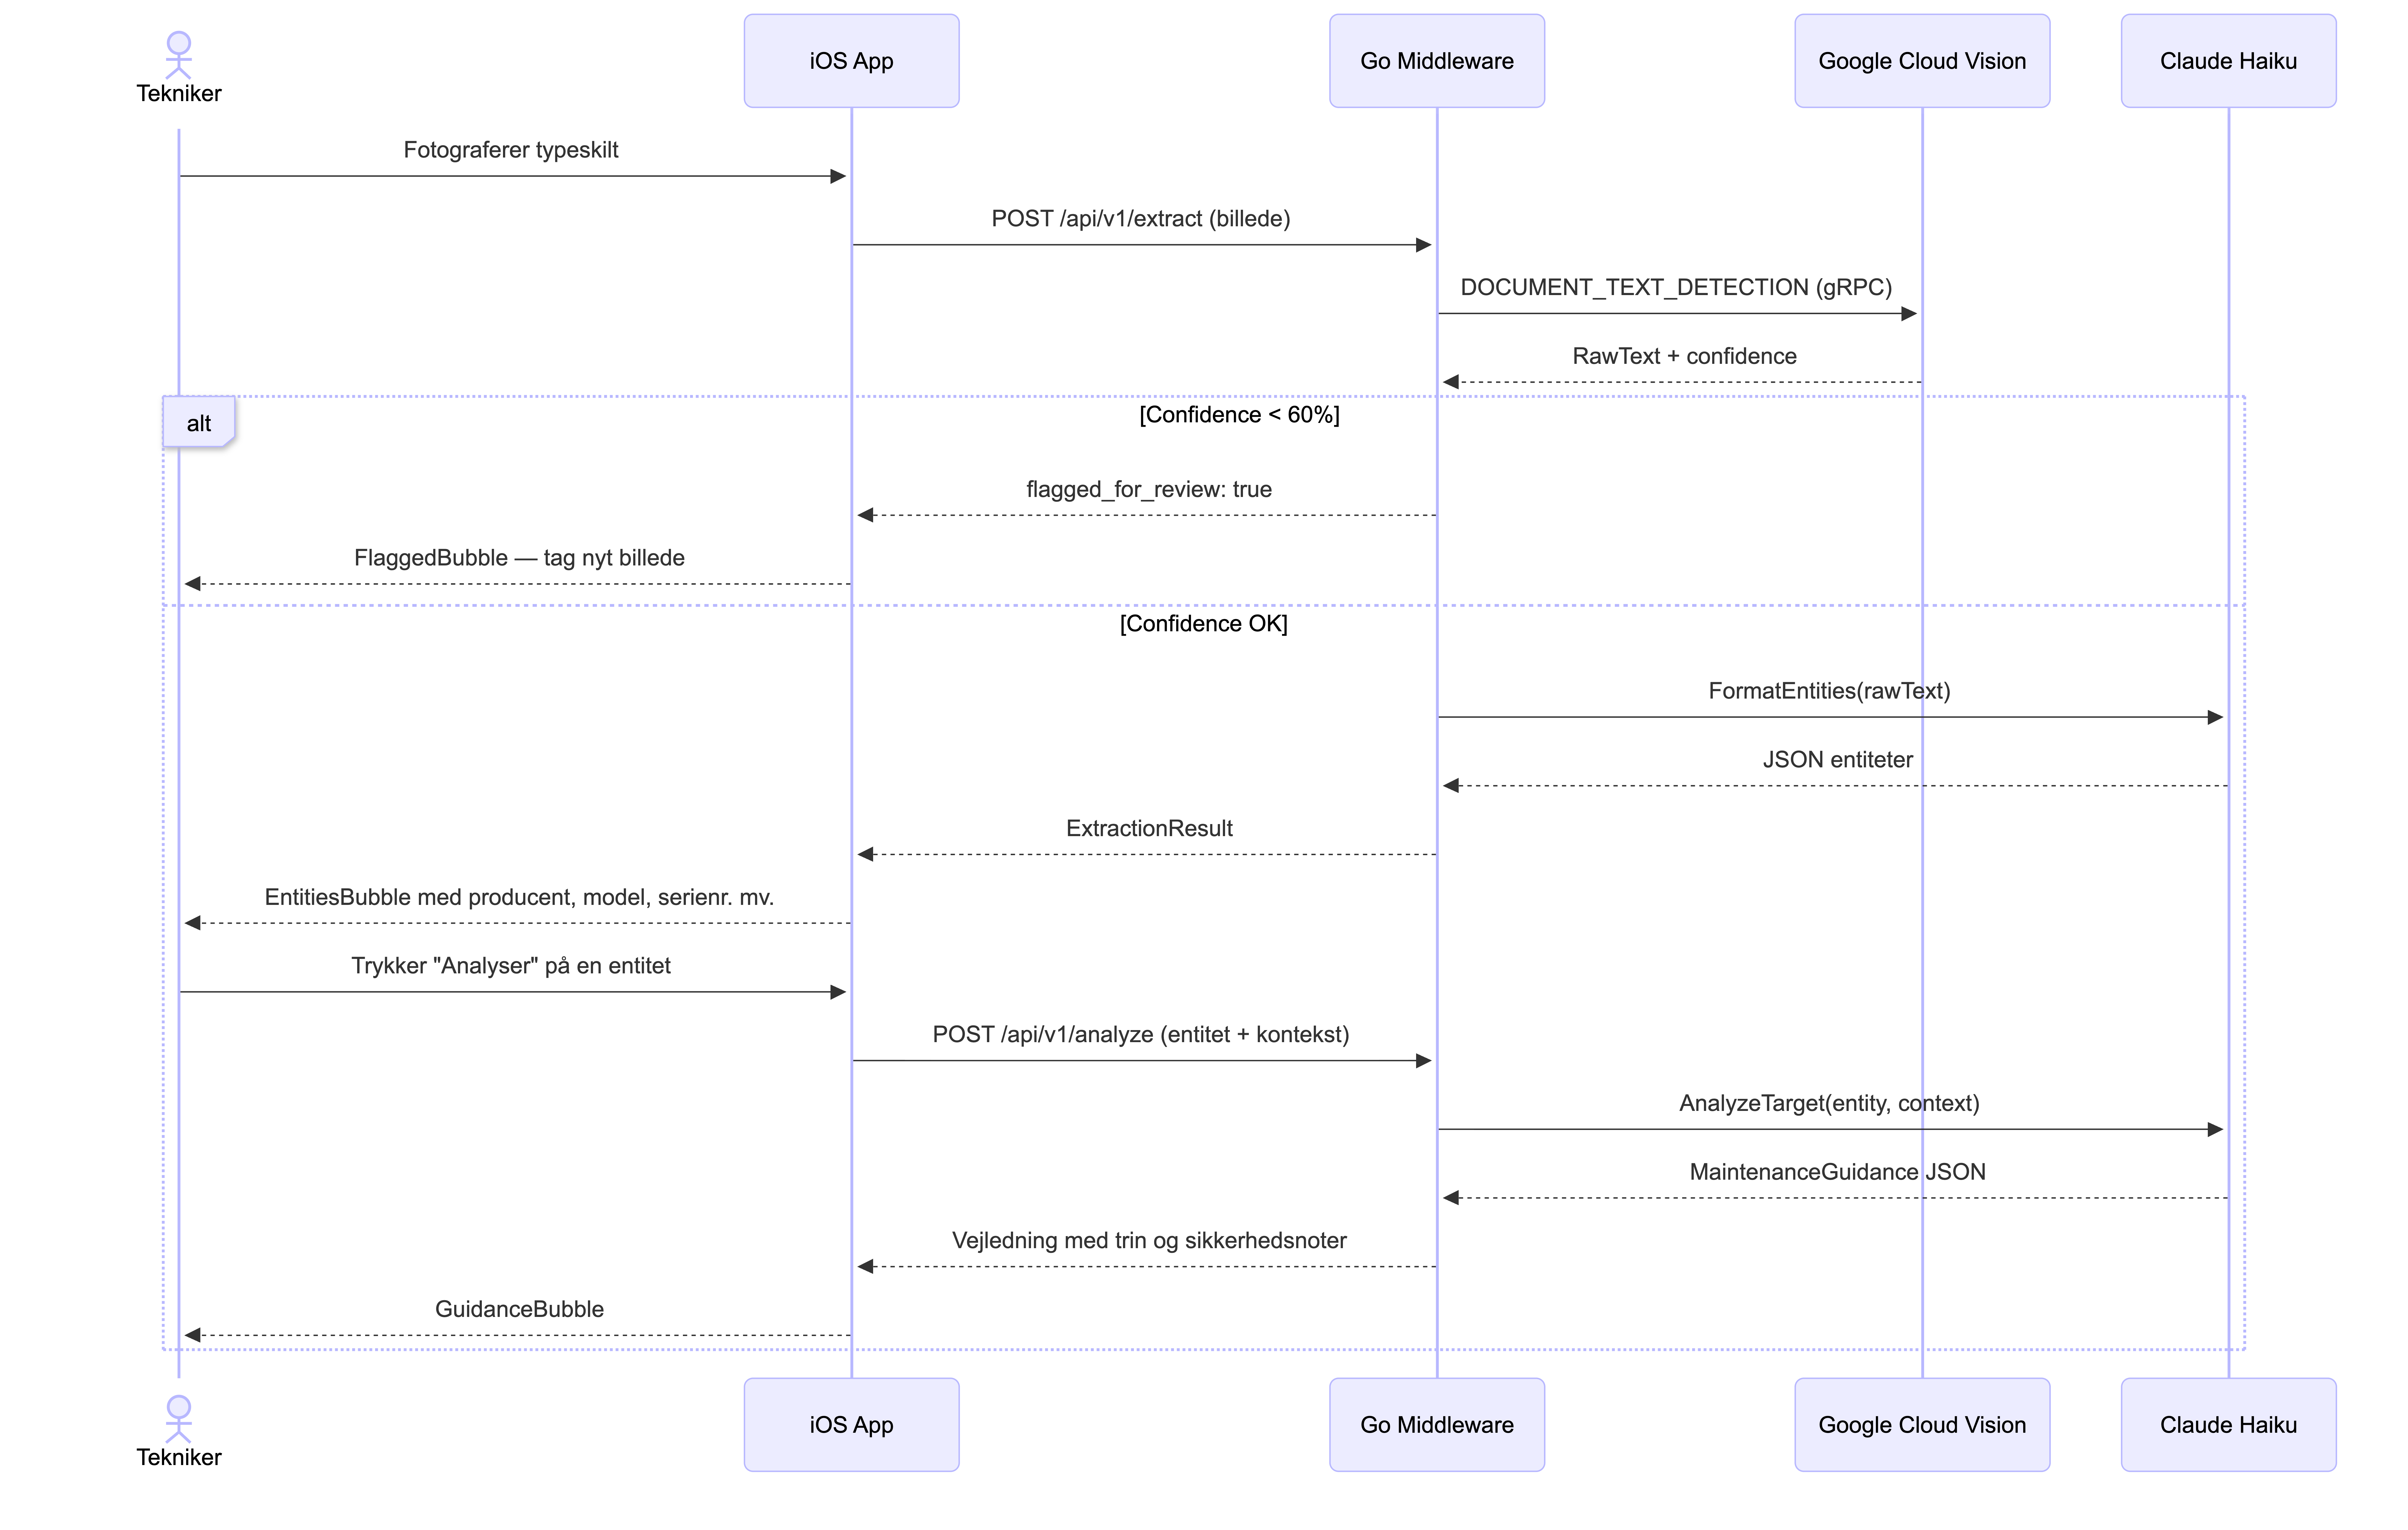
\includegraphics[width=\textwidth]{figures/AppFlowDiagram.png}
  \caption{Sekvensdiagram for billedbaseret udtræk}
  \label{fig:flow-image}
\end{figure}

Forløbet er som følger:

\begin{enumerate}
  \item Teknikeren optager et billede via \texttt{ImagePicker}, som returnerer et \texttt{UIImage}-objekt til \texttt{CameraViewModel}
  \item \texttt{ChatViewModel.extractImage()} konverterer billedet til JPEG-data (80\% komprimering) og sender det som \texttt{multipart/form-data} til \texttt{POST /api/v1/extract} med en timeout på 60 sekunder
  \item \texttt{NewExtractHandler} i Go parser form-data og sender billedets rå bytes til Google Cloud Vision via \texttt{BatchAnnotateImages}-kaldet med \texttt{DOCUMENT\_TEXT\_DETECTION}-feature
  \item Vision returnerer en \texttt{FullTextAnnotation} med tekst og symbol-confidence scores. Funktionen \texttt{averageSymbolConfidence()} traverserer annotationshierarkiet (side → blok → paragraf → ord → symbol) og beregner en gennemsnitlig confidence-score
  \item Hvis confidence er under tærsklen på 60\% (\texttt{confidenceThreshold = 0.60}), returneres resultatet øjeblikkeligt med \texttt{FlaggedForReview: true} uden at kalde Claude
  \item Ved tilstrækkelig confidence sendes råteksten til \texttt{ClaudeClient.FormatEntities()}, som via \texttt{extractSystemPrompt} instruerer modellen til at returnere strukturerede entiteter som JSON
  \item \texttt{cleanJSONResponse()} udtrækker JSON-objektet fra svaret og trimmer eventuelle markdown-wrappers
  \item Det dekodede \texttt{ExtractionResult} returneres til iOS-klienten, som renderer resultatet som en \texttt{EntitiesBubble} eller — ved lav confidence — en \texttt{FlaggedBubble}
\end{enumerate}

\section{Dataflow: Videobaseret udtræk}
\label{sec:dataflow-video}

Videobehandlingen følger et udvidet pipeline der inkluderer frame-udtræk via ffmpeg:

\begin{enumerate}
  \item Teknikeren optager en video og panorerer kameraet henover maskinlabelen. Videofilen (mp4-format) sendes som \texttt{multipart/form-data} til \texttt{POST /api/v1/extract} med en timeout på 120 sekunder
  \item \texttt{processVideo()} i \texttt{video.go} gemmer videodata i en midlertidig mappe og kalder ffmpeg via \texttt{exec.CommandContext}: \texttt{ffmpeg -i video.mp4 -vf fps=1 frame\_\%03d.jpg}
  \item Hvert ekstraheret frame sendes individuelt til Google Cloud Vision OCR
  \item Tekstresultaterne fra alle frames aggregeres med frame-headers (\texttt{"--- Frame N ---"}) og en gennemsnitlig confidence beregnes på tværs af alle gyldige frames
  \item Det aggregerede tekstindhold behandles af Claude som én samlet streng, identisk med billedflowet
\end{enumerate}

Den midlertidige mappe slettes automatisk via \texttt{defer os.RemoveAll(tempDir)} uanset udfaldet af behandlingen.

\section{Dataflow: AI-vejledning}
\label{sec:dataflow-analyze}

Når teknikeren trykker \textit{Analyser} på en entitet i \texttt{EntitiesBubble}, trigges følgende flow:

\begin{enumerate}
  \item \texttt{ChatViewModel.analyzeEntity()} sender en \texttt{AnalyzeRequest} som JSON til \texttt{POST /api/v1/analyze} med \texttt{target\_label}, \texttt{target\_value}, \texttt{machine\_model} (udledt fra kontekst-entiteterne) og alle øvrige entiteter som baggrundskontekst
  \item \texttt{NewAnalyzeHandler} validerer input og videresender til \texttt{ClaudeClient.AnalyzeTarget()}
  \item Claude instrueres via \texttt{analyzeSystemPrompt} til at generere struktureret vejledning med minimum tre vejledningsskridt, to sikkerhedsnoter og et \texttt{uncertainty\_level} (\texttt{"low"}, \texttt{"medium"} eller \texttt{"high"})
  \item Sproget for vejledningen styres af \texttt{language}-feltet i requesten (\texttt{"da"} eller \texttt{"en"}), som bestemmer hvilken sproglig instruktion der tilføjes prompten
  \item Den dekodede \texttt{MaintenanceGuidance} returneres og renderes som en \texttt{GuidanceBubble} i iOS-klienten
\end{enumerate}

\section{Fejlhåndtering}
\label{sec:fejlhaandtering}

Systemet implementerer en gennemgående fejlhåndteringsstrategi på tværs af klient og server.

På \textbf{serversiden} returnerer alle handlers strukturerede JSON-fejlsvar med HTTP-statuskoder. Input valideres eksplicit inden AI-kald, så ugyldige requests afvises med \texttt{400 Bad Request} før eksterne services kontaktes.

På \textbf{klientsiden} implementerer \texttt{ChatViewModel} et \texttt{RetryContext}-mønster: enhver fejlbesked gemmer den originale kontekst (billeddata, video-URL eller entitet), så brugeren kan prøve igen med ét tryk uden at gentage hele flowet fra start. Dette håndteres via \texttt{ErrorBubble}-komponenten, der viser en meningsfuld fejlbesked og en \textit{Prøv igen}-knap.

\section{Deployment}
\label{sec:deployment}

Go-serveren deployes til DTU-serveren via et automatiseret shell-script (\texttt{deploy.sh}), der udfører følgende trin i rækkefølge:

\begin{enumerate}
  \item Køring af samtlige Go-unit tests (\texttt{go test ./...}) — scriptet afbrydes ved testfejl
  \item Cross-kompilering til Linux/amd64: \texttt{GOOS=linux GOARCH=amd64 go build -o arkyn-server}
  \item Stop af den kørende systemd-service via SSH
  \item Kopiering af den nye binær til serveren via \texttt{scp}
  \item Genstart af service og verifikation af servicestatus
\end{enumerate}

Serverens konfiguration — herunder API-nøgler til Anthropic og Google Cloud — læses udelukkende fra miljøvariabler (\texttt{ANTHROPIC\_API\_KEY}, \texttt{GOOGLE\_APPLICATION\_CREDENTIALS}), der aldrig indgår i versionsstyringen.
